% GDZ PPN236018647,native492;HKUST493;manuscript first sheet.
\clearpage\SourceLeaf{492}\NoSourceHead
\begingroup\itshape
\begin{center}1796\end{center}
\noindent\makebox[1.2em][l]{\(\ast\)}\underline{Principia quibus innititur sectio circuli,}\\
\hspace*{2em}\underline{ac divisibilitas eiusdem geometrica in}\\
\hspace*{2em}\underline{septendecim partes} \&c.\hfill Mart 30\quad Brunsv.

\medskip
\noindent\makebox[1.2em][l]{\(\ast\)}\underline{Numerorum primorum non omnes}\\
\hspace*{2em}\underline{numeros infra ipsos residua quadratica}\\
\hspace*{2em}\underline{esse posse demonstratione munitum.}
\begin{flushright}Apr. 8.\quad Ibid.\end{flushright}

\noindent\underline{Formulae pro cosinibus angulorum periphe}\\
\hspace*{2em}\underline{riae submultiplorum expressionem gene-}\\
\hspace*{2em}\underline{raliorem \rlap{\raisebox{1.1ex}[2ex][0pt]{\scriptsize non}}admittent nisi in duab. periodis}
\begin{flushright}Apr. 12.\quad Ibid\end{flushright}

\noindent\makebox[1.2em][l]{\tikz[baseline=-.1ex,x=1ex,y=1ex]{\draw[line width=.45pt] (0,0)--(.45,.55)--(.45,1.15); \draw[line width=.45pt] (.45,.55)--(1.05,.2);}}\underline{Amplificatio normae residuorum ad residua}\\
\hspace*{2em}\underline{et mensuras non indivisibiles.}
\begin{flushright}Apr. 29\quad Gotting.\end{flushright}

\noindent Numeri cuiusvis divisibilitas varia in binos primos
\begin{flushright}Mai. 14\quad Gott\end{flushright}

\noindent\makebox[1.2em][l]{\tikz[baseline=-.1ex,x=1ex,y=1ex]{\draw[line width=.45pt] (0,0)--(.45,.55)--(.45,1.15); \draw[line width=.45pt] (.45,.55)--(1.05,.2);}}Coefficientes aequationum per radicum potestates\\
\hspace*{2em}additas facile dantur\hfill Mai. 23 Gott.

\medskip
\noindent Transformatio seriei \(1-2+8-64\,{.}\) in fractionem\\
\hspace*{2em}continuam
\begin{center}
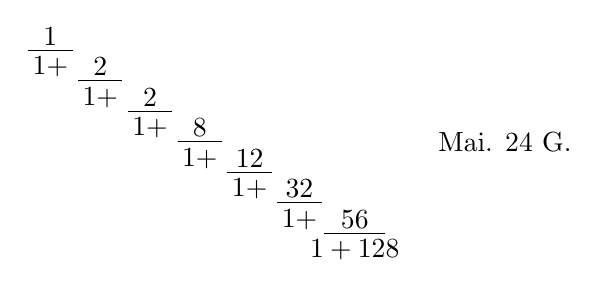
\begin{tikzpicture}[x=1em,y=1em,baseline=(current bounding box.center)]
\node[inner sep=0] at (0,0) {\(1\)};
\draw (-.8,-.5)--(.8,-.5);
\node[inner sep=0] at (0,-1.1) {\(1+\)};
\node[inner sep=0] at (1.8,-1.1) {\(2\)};
\draw (1,-1.6)--(2.6,-1.6);
\node[inner sep=0] at (1.8,-2.2) {\(1+\)};
\node[inner sep=0] at (3.6,-2.2) {\(2\)};
\draw (2.8,-2.7)--(4.4,-2.7);
\node[inner sep=0] at (3.6,-3.3) {\(1+\)};
\node[inner sep=0] at (5.4,-3.3) {\(8\)};
\draw (4.6,-3.8)--(6.2,-3.8);
\node[inner sep=0] at (5.4,-4.4) {\(1+\)};
\node[inner sep=0] at (7.2,-4.4) {\(12\)};
\draw (6.4,-4.9)--(8.0,-4.9);
\node[inner sep=0] at (7.2,-5.5) {\(1+\)};
\node[inner sep=0] at (9,-5.5) {\(32\)};
\draw (8.2,-6)--(9.8,-6);
\node[inner sep=0] at (9,-6.6) {\(1+\)};
\node[inner sep=0] at (11,-6.6) {\(56\)};
\draw (9.9,-7.1)--(12.1,-7.1);
\node[inner sep=0] at (11,-7.7) {\(1+128\)};
\node[anchor=west,inner sep=0] at (14,-3.8) {Mai. 24 G.};
\end{tikzpicture}
\end{center}
\[
1-1+1.3-1.3.7+1.3.7.15=
\]
\begin{center}
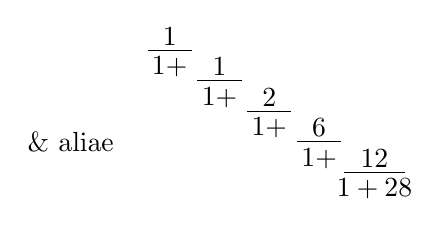
\begin{tikzpicture}[x=1em,y=1em,baseline=(current bounding box.center)]
\node[inner sep=0] at (0,0) {\(1\)};
\draw (-.8,-.5)--(.8,-.5);
\node[inner sep=0] at (0,-1.1) {\(1+\)};
\node[inner sep=0] at (1.8,-1.1) {\(1\)};
\draw (1,-1.6)--(2.6,-1.6);
\node[inner sep=0] at (1.8,-2.2) {\(1+\)};
\node[inner sep=0] at (3.6,-2.2) {\(2\)};
\draw (2.8,-2.7)--(4.4,-2.7);
\node[inner sep=0] at (3.6,-3.3) {\(1+\)};
\node[inner sep=0] at (5.4,-3.3) {\(6\)};
\draw (4.6,-3.8)--(6.2,-3.8);
\node[inner sep=0] at (5.4,-4.4) {\(1+\)};
\node[inner sep=0] at (7.4,-4.4) {\(12\)};
\draw (6.3,-4.9)--(8.5,-4.9);
\node[inner sep=0] at (7.4,-5.5) {\(1+28\)};
\node[anchor=east,inner sep=0] at (-2,-3.8) {\& aliae};
\end{tikzpicture}
\end{center}
\endgroup

